\documentclass{beamer}
\usepackage[utf8]{inputenc}
\usepackage[danish, english]{babel}
\usepackage{beamerthemesplit}
\usepackage{color}

% Math support
\usepackage{amssymb}
\usepackage{amsmath}

\title[OCamlCSP]{
  OCamlCSP - A concurrency library for OCaml
}
\author[Ramón Soto]{
  Ramón Soto Mathiesen
}
\institute{Computer Science Department \\ Copenhagen University}
\date{Tuesday, 25$^{th}$ August 2009}

\definecolor{kugreen}{RGB}{50,93,61}
\definecolor{kugreenlys}{RGB}{132,158,139}
\definecolor{kugreenlyslys}{RGB}{173,190,177}
\definecolor{kugreenlyslyslys}{RGB}{214,223,216}
\setbeamercovered{transparent}
\mode<presentation> {
 \usetheme{PaloAlto}
 \usecolortheme[named=kugreen]{structure}
 \useinnertheme{circles}
 \usefonttheme[onlymath]{serif}
 \setbeamercovered{transparent}
 \setbeamertemplate{blocks}[rounded][shadow=true]
}
\logo{
\includegraphics[width=1cm]{figures/B_NAT_cmyk.pdf}}

% Macros
\newcommand{\green}[1] {\textcolor{kugreen}{#1}}

% Line breaks between paragraphs instead of indentation
\parindent=0pt
\parskip=8pt plus 2pt minus 4pt

\begin{document}

\begin{frame}
 \titlepage
\end{frame}

\begin{frame}
 \frametitle{Contents}
 \setcounter{tocdepth}{2}
 \tableofcontents
\end{frame}

\section[Intro]{Introduction to OcamlCSP}
\begin{frame}
  \frametitle{Introduction to OcamlCSP}
  \begin{itemize}
  \item Is a concurrency library for the functional language OCaml.
  \item It is based on Communicating Sequential Processes by Tony Hoare and
    a other existing libraries that are based on CSP (PyCSP, JCSP, CPPCSP2).
  \item We provide overlapping I/O and concurrency.
  \item We don't provide true parallelism.
  \end{itemize}
\end{frame}

\section[CSP]{Communicating concurrent processes}
\begin{frame}
  \frametitle{Communicating concurrent processes}
  \begin{itemize}
    \item Each process has it's own encapsulated data structures and algorithms.
    \item The only way to communicate between processes it's between synchronised
      messages.
    \item Each process should be thought as a piece of hardware placed on a
      circuit board and the CSP network as the Electrical network. This way you
      can make small components, which are easy to prove correctness, and by
      combining them together you get bigger processes/CSP networks.
  \end{itemize}
\end{frame}

\section[API]{Application programming interface design}
\begin{frame}
  \frametitle{Application programming interface design}
  \begin{itemize}
    \item Processes.
      \begin{itemize}
        \item Hierarchical model.
      \end{itemize}
    \item Channels. 
      \begin{itemize}
        \item Any-to-any.
      \end{itemize}
    \item Alternation (Guards).
      \begin{itemize}
        \item General choice (CSP).
        \item No PRI ALT (Ambiguous definition in Occam).
      \end{itemize}
    \item Poison.
      \begin{itemize}
        \item No propagation.
      \end{itemize}
    \item Permission.
      \begin{itemize}
        \item Compile time error.
      \end{itemize}
  \end{itemize}
\end{frame}

\begin{frame}[fragile]
  \frametitle{Processes}
  CSP syntax, P in parallel with Q:
    \[P \parallel Q\]
  How do we represent two processes running concurrent:
\scriptsize
\begin{verbatim}
Csp.parallel [
    (fun () -> ...);
    (fun () -> ...);
]
\end{verbatim}
\normalsize
\green{Remark:} The only way to retrieve a value from the processes running in
parallel is to create internal channels ...
\end{frame}

\begin{frame}[fragile]
  \frametitle{Processes}
    \[(c_1\,?\,x \to SKIP \parallel c_2\,?\,y \to SKIP); c_3\,!\,(x + y)\]
\scriptsize
\begin{verbatim}
let c1' = Csp.new_channel () in
let c2' = Csp.new_channel () in
parallel [
    (fun () -> Csp.write c1' (Csp.read c1));
    (fun () -> Csp.write c2' (Csp.read c2));
    (fun () -> Csp.write c3 (Csp.read c1' + Csp.read c2'));
]
\end{verbatim}
\normalsize
Even though the ideal would be returning a tuple, but ...
\scriptsize
\begin{verbatim}
let (x, y) = parallel2 (
    (fun () -> Csp.read c1), 
    (fun () -> Csp.read c2)
) in Csp.write c3 (x + y)
\end{verbatim}
\normalsize
\end{frame}


\begin{frame}[fragile]
  \frametitle{Channels}
  CSP syntax, on (channel) $c$ output (value of) $e$ and on (channel) $c$ input
  to $x$:
    \[c\,!\,e \to ...\]
    \[c\,?\,x \to ...\]
  Our representation would be:
\scriptsize
\begin{verbatim}
Csp.write c e; ...
let x = Csp.read c in ...
\end{verbatim}
\normalsize
\end{frame}

\begin{frame}
  \frametitle{Channels}
  One-to-one channel represented as a state machine, only one process can read
  to it and another can write to it:
  \begin{figure}[htp]
    \begin{center}
      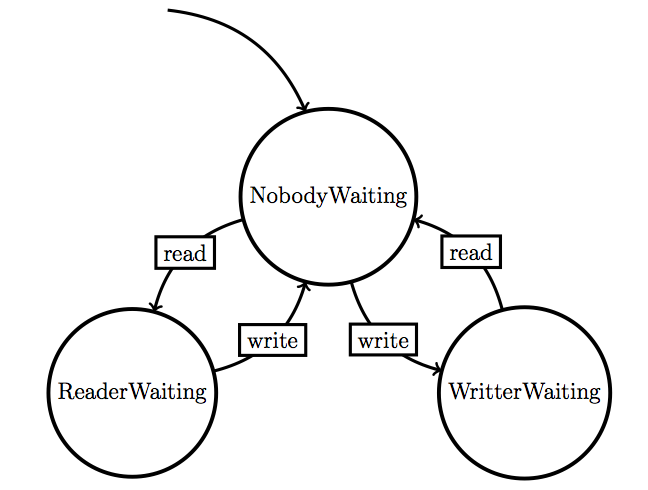
\includegraphics[width=4.5cm,keepaspectratio=true]{figures/channels.png}
    \end{center}
  \end{figure}
  Expanding one-to-one channel to a any-to-any channel is done by adding a queue
  of readers and a queue of writers.

  \green{Remark:} We ensure that no process will be starved. 
\end{frame}


\begin{frame}[fragile]
  \frametitle{Alternation (Guards)}
  CSP syntax, $c_1?x$ choice $c_2?y$ choice $c_3!e$:
  \[(c_1\,?\,x \to ...\ |\ c_2\,?\,y \to ...\ |\ c_3\,!\,e \to ...)\]
  Our representation would be:
\scriptsize
\begin{verbatim}
Csp.select [
    Csp.read_guard c1 (fun x -> ...);
    Csp.read_guard c2 (fun y -> ...);
    Csp.write_guard c3 e (fun () -> ...);
]
\end{verbatim}
\normalsize
\end{frame}

\begin{frame}[fragile]
  \frametitle{Alternation (Guards)}
  We provide guarded processes, where the action is carried out whenever
  the guarded is chosen, this removes the responsibility from the developer,
  as in most of the other libraries, the developer receives the index value
  from the list of guards and it's his responsibility to perform the desired
  action.

  CSP syntax, $c?x$ or $c?x$ (non-deterministic):
  \[(c\,?\,x \to ...) \sqcap (c\,?\,x \to ...)\]
  We have the possibility to have several guarded processes to wait on the same
  channel. Based on the implementation, we could actually get internal choice,
  where the pick of the process not has to be fair (non-deterministic).

  By combining external and internal choice, we will have the general choice
  from CSP.
\end{frame}


\begin{frame}[fragile]
  \frametitle{Poison}
  CSP syntax, none:
  \[\]
  Our representation:
\scriptsize
\begin{verbatim}
Csp.poison c 
\end{verbatim}
\normalsize
We need some kind of mechanism to shut down the CSP network correctly,
we couldn't come up with a better idea than the one they use in most of the
other CSP libraries. So we also decided to implement Poison. Which means, that
once a channel is poisoned it can never get back to normal state and if a
process reads or writes to a poisoned channel, it throws a poison exception,
which can be handled to propagate the poison to other channels. In PyCSP, this
is done automatically.
\end{frame}


\begin{frame}[fragile]
  \frametitle{Permission}
  CSP syntax, none:
  \[\]
  Our representation:
\scriptsize
\begin{verbatim}
let rec p c () =
  let _ = Csp.read (Csp.read_poison_only c); p c ()
\end{verbatim}
\normalsize
  Because we implemented poison, we would like to ensure that some part of our
  CSP networks will not be able to shutdown the entire network.

  By adding channel permissions, we can ensure that a process don't read, write
  or poison a specified channel (compiler error).
\end{frame}

\begin{frame}
  \frametitle{Permission}
  \begin{figure}[h]
    \centering
    \begin{tabular}{c|c|c|l}
      Read & Write & Poison & Function \\
      \hline
      0 & 0 & 0 & - \\
      0 & 0 & 1 & poison\_only \\
      0 & 1 & 0 & write\_only \\
      0 & 1 & 1 & write\_poison\_only \\
      1 & 0 & 0 & read\_only \\
      1 & 0 & 1 & read\_poison\_only \\
      1 & 1 & 0 & read\_write\_only \\
      1 & 1 & 1 & (default) \\
    \end{tabular}
  \end{figure}
\end{frame}


%\begin{frame}
%  \frametitle{OcamlCSP Utility Library}
%  CSPU
%\end{frame}


\section[Legoland]{OcamlCSP Component Library (Legoland)}
\begin{frame}[fragile]
  \frametitle{OcamlCSP Component Library (Legoland)}
  \begin{figure}[htp]
    \begin{center}
      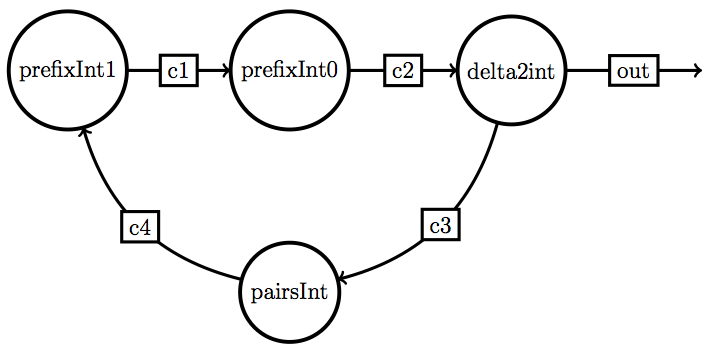
\includegraphics[width=8cm,keepaspectratio=true]{figures/fib.png}
    \end{center}
  \end{figure}
\tiny
\begin{verbatim}
let fibonacciInt o () =
  let c1 = Csp.new_channel () in
  let c2 = Csp.new_channel () in
  let c3 = Csp.new_channel () in
  let c4 = Csp.new_channel () in
    Csp.parallel [
      prefixint (bii 1) c4 c1 ;
      prefixint (bii 0) c1 c2 ;
      delta2int c2 o c3;
      pairsInt c3 c4
    ]
\end{verbatim}
\normalsize
\end{frame}

\begin{frame}[fragile]
  \frametitle{OcamlCSP Component Library (Legoland)}
  \begin{figure}[htp]
    \begin{center}
      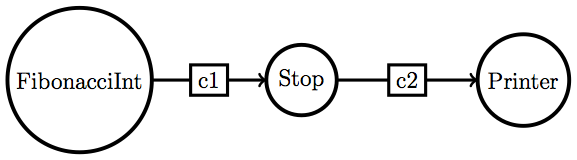
\includegraphics[width=8cm,keepaspectratio=true]{figures/fib2.png}
    \end{center}
  \end{figure}
\tiny
\begin{verbatim}
let _ = 
  let c1 = Csp.new_channel () in
  let c2 = Csp.new_channel () in
      try Csp.parallel [
        fibonacciInt c1;
        stop 42 c1 c2;
        printer c2
      ] with Csp.PoisonException -> ()
\end{verbatim}
\normalsize
\end{frame}

%\begin{frame}[fragile]
%  \frametitle{Simple example (even numbers)}
%  \tiny
%\begin{verbatim}
%let rec counter n o () =
%  Csp.write o n; counter (n+1) o ()
%
%let rec double i o () =
%  let x = Csp.read i in
%  Csp.write o (x*2); double i o ()
%
%let rec print i () =
%  print_endline(string_of_int (Csp.read i)); print i ()
%
%let even_numbers o () =
%  let c = Csp.new_channel () in
%    Csp.parallel [
%      counter 1 c;
%      double c o;
%    ]
%
%let _ =
%  let c = Csp.new_channel () in
%    Csp.parallel [
%      even_numbers c;
%      print c
%    ]
%\end{verbatim}
%  \normalsize
%\end{frame}


\section[Comparison]{Comparison to other CSP Libraries}
\begin{frame}
  \frametitle{Comparison to other CSP Libraries}
  \begin{figure}[h]
    \centering
    \begin{tabular}{l|c|c|c|c}
      Constructs & PyCSP & JCSP & CPPCSP2 & OcamlCSP \\
      \hline
       True parallelism\footnote{Multiple CPUs/cores.} & No & No & Yes & No \\
       Alternation & Yes & Yes & Yes & Yes\footnote{No PRI ALT implementation,
         but combination of read/write guards.} \\
       Read guards & Yes & Yes & Yes & Yes \\
       Write guards & No & Yes & No & Yes \\
       Guarded processes & No & No & No & Yes \\
       Channel any-to-any & Yes & Yes & Yes & Yes \\
       Channel poison & Yes & Yes & Yes & Yes \\
       Channel permissions & Yes & Yes & Yes & Yes\footnote{Disallow
         read/write/poison from/to/of channel at compile time.} \\
       Type system & No & No\footnote{JCSP cast objects.} & Yes & Yes \\
    \end{tabular}
  \end{figure}
\end{frame}

\begin{frame}[fragile]
  \frametitle{Performance test OcamlCSP vs PyCSP}
  \tiny
\begin{verbatim}
open Cspu
open Legoland

let consumer i () =
  let n = 5000 in
  (* let ts = Unix.time in *)
  let ts = Unix.gettimeofday in
  let t1 = ts () in
    for j = 0 to n do
      Csp.read i
    done;
    let t2 = ts () in
    let dt = t2 -. t1 in
    let tcha = dt /. (4.0 *. float_of_int n) in
      Printf.printf "DT = %f.\nTime per ch : %f/(4*%d) = %f s = %f us\n"
        dt dt n tchan (tchan *. 1000000.0);
      Printf.printf "consumer done, poisoning channel";
      Csp.poison i
\end{verbatim}
  \normalsize
\end{frame}

\begin{frame}[fragile]
  \frametitle{Performance test OcamlCSP vs PyCSP}
  \tiny
\begin{verbatim}
from common import *
import time

def CSP_Commstime_ConsumerFunc(cin):
    "Commstime consumer process"
    N = 5000
    ts = time.time
    t1 = ts()
    cin()
    t1 = ts()
    for i in range(N):
        cin()
    t2 = ts()
    dt = t2-t1
    tchan = dt / (4 * N)
    print "DT = %f.\nTime per ch : %f/(4*%d) = %f s = %f us" % \
          (dt, dt, N, tchan, tchan * 1000000)
    print "consumer done, poisoning channel"
    poisonChannel(cin)
\end{verbatim}
  \normalsize
\end{frame}

\begin{frame}[fragile]
  \frametitle{Performance test OcamlCSP vs PyCSP}
OcamlCSP:
\tiny
\begin{verbatim}
DT = 0.145585.
Time per ch : 0.145585/(4*5000) = 0.000007 s = 7.279253 us
consumer done, poisoning channel
\end{verbatim}
\normalsize
PyCSP(*):
\tiny
\begin{verbatim}
DT = 2.660773.
Time per ch : 2.660773/(4*5000) = 0.000133 s = 133.038640 us
consumer done, poisoning channel
\end{verbatim}
\normalsize
(*) The PyCSP version is executed with CSP-Builder.
\end{frame}


\section[Web proxy]{Web proxy}
\begin{frame}
  \frametitle{Web proxy}
  \begin{itemize}
    \item Gateway
      \begin{itemize}
        \item Accept loop
          \begin{itemize}
            \item Handler
          \end{itemize}
        \item Cache
      \end{itemize}
  \end{itemize}
  \begin{itemize}
    \item Handler (client socket) 
      \begin{itemize}
        \item http\_downloader (server socket)
          \begin{itemize}
          \item socket\_downloader
          \end{itemize}
      \end{itemize}
  \end{itemize}
  \begin{itemize}
    \item socket\_downloader
      \begin{itemize}
        \item delta
          \begin{itemize}
            \item client socket
            \item registrator (cache)
          \end{itemize}
      \end{itemize}
  \end{itemize}
\end{frame}


\section[Demo]{Demonstration (Web proxy)}
\begin{frame}
  \frametitle{Demonstration (Web proxy)}
  \begin{itemize}
    \item Start the web proxy.
    \item Choose two mirrors from Gentoo (Denmark and Thailand).
    \item Enable proxy to show how cache work.
    \item Retrieve concurrent two big files from mirrors where the slowest,
      Thailand, is chosen first. (Non blocking I/O).
  \end{itemize}
\end{frame}

\end{document}
